 
\subsection{Experiment setup}

In RQ1, in order to check the accuracy of the benchmark proposed in this project, 
we first compare the context switch time measured by prior benchmarks and the proposed ones on local PC.
For local measurements, we use an Ubuntu 20.04-64bit machine with Intel(R) Core(TM) i7-8750H CPU @ 2.20GHz processor and 12GB RAM.
Then in RQ2, we will use the proposed benchmark to measure the context switch time in Google Cloou Function, 
which is a mainstream cloud platform to provide serverless computing.

% We implement the benchmarks on Google Cloud, which is a mainstream cloud platform to provide serverless functions. 
% For local measurements, we use an Ubuntu 20.04-64bit machine with Intel(R) Core(TM) i7-8750H CPU @ 2.20GHz processor and 12GB RAM.
% We plan to do experiments in more types of machines and operating systems to show the generality of the benchmark.

%\subsection{Factors impacting context switches in serverless environment}
% TODO

\subsection{RQ1: Measuring local context switches}

% All the previous benchmarks\cite{cs-web,cs-datasize,cs-lmbench,cs-pipes} are implemented in C language.
% However, currently Google Cloud only supports functions written in Node.js, Go, Java, Python and Ruby.
% Considering that Python is one of the most popular languages, rewriting the prior benchmarks in Python and examining its correctness in local PC is important.

% The context switch time measured by the first three benchmarks in local PC is usually among 2us from Table~\ref{tab:experiment1}.
% In the first row, pipe, condition var and lmbench refers to methods listed in Section 2 respectively.
% However, when it's rewritten by Python, the measured time is 10 times larger than previous results. 
% The reason might be that extra execution is added to the time measurement when translating the language.
% What's more, the C programs execute faster as compiled programs while Python executes slower due its interpreted programs, 
% and these extra execution time is more obvious when using python. 
% Therefore, we plan to measure the time variation induced by Python on local computers and scale the measured time in cloud accordingly.
% Table~\ref{tab:experiment1} shows that the context switch time measured by the pipe method written in Python is about 17.14 times larger than measuring in C programs.
% In our further experiment in cloud, we'll take the python measured time divided by 17.14 as the context switch time.

% \subsubsection{Context switches time with different benchmarks}
% We write our own benchmark in Python, and we want to compare it with previous benchmarks to check its correctness. 
% Therefore, we show the results for thread context switching for with pingpong method, condition var and process context switching with lmbench and pid sum, and perf (+pidstat/vmstat?)
% For lmbench, we choose xxx size. We run 100 times and get the median value and variance. And we draw them below in the figures. - bar plot, median and variance

% 1. Compare context switch between processes and threads.

% 2. Compare context switch between programming languages. (Pay attention to divide Python by 10)

% \subsubsection{Context switch time with different number of processes}

% I can't guarantee the size of the process

In this research question, we want to compare our benchmarks in Python with previous benchmarks to check its correctness. 
For each benchmark, we run 200 times and plot the results.
Fig.\ref{fig:thread_local} shows the context switch time measured by 5 benchmarks on local PC. 
\emph{ThreadpingC} is the original \emph{Pingpong pipes}\cite{cs-pipes,cs-web} written in C.
\emph{ThreadCondC} is the original \emph{Condition var}\cite{cs-web} written in C.
\emph{ThreadpingP} is the thread benchmark proposed in this project written in Python.
These first three benchmarks measure the thread context switch time.
\emph{Lmbench} is the \emph{Lmbench}\cite{cs-lmbench} written in C.
\emph{ProcRing} is the process benchmark proposed in this project written in Python.a
The last two measure the process context switch time. 
 
The first two bars show that the thread context switch time measured by benchmarks in C language is around 2.3/2.4 microseconds and the coefficient of variation is very low. 
The time measured by the benchmarks written in Python, however, is almost 15-20x longer than C programs. 
This might due to the following reasons. 1) Python's execution speed is slower than compiled language like C, as Python is interpreted at runtime instead of being compiled to native code at compile time. 
2) During the slow execution of Python, there might be more than 2 context switches happening.

As for the first reason, 

This may make Python slower than compiled languages like C. Also, there is comparatively large variance in third benchmark. It may due to programming languages itself or some code modifications during my implementation in a new language. But this is acceptable as its Coefficient of variation  is lower than 10%





Therefore, we show the results for thread context switching for with pingpong method, condition var and process context switching with lmbench and pid sum, and perf (+pidstat/vmstat?)
For lmbench, we choose xxx size. We run 100 times and get the median value and variance. And we draw them below in the figures. - bar plot, median and variance


\subsection{Measuring context switches in the cloud}

\subsubsection{Non-parametric analysis among different memories}

We first collect 200 data for each memory setting. And then we perform xxx method to check the normality. 
-> show the results for checking normallity

Because it's not normal distribution, we then use non-parametric method to determine the number of experiment times. 



We create functions with different memory allocated and measure the context switch time with the Ping pong pipes method.
For each memory configuration we run 10 times and get the average of the calculated time. 
We also notion that the variation induced by Python language has already been considered and the value shown in Table~\ref{tab:cloud} is processed.
We notice that if the allocate memory is 128GB, the context switch time is remarkably higher than the other configurations.
And we plan to look deeper into this in the future.

% \begin{center}
%     \begin{table}
%     \begin{tabular}{||c c c c c||} 
%      \hline
%      Benchmark & Pingpong& Condition Var & Lmbench & Pipe(python) \\ 
%      \hline
%      Time(/us) & 1.96 & 2.29 & 1.78 & 33.6\\ 
%      \hline
%     \end{tabular}
%     \caption{\label{tab:experiment1}Context switch time by different benchmarks}
% \end{table}
% \end{center}

% \begin{center}
%     \begin{table}
%     \begin{tabular}{||c c c c||} 
%      \hline
%       Memory(/MB) & 128 & 256 & 512 \\ 
%      \hline
%      Time(/us) & 81.11 & 33.96 & 36.17 \\ 
%      \hline
%     \end{tabular}
%     \caption{\label{tab:cloud}Context switch time in functions with different memories }
% \end{table} 
% \end{center}




% Figure~\ref{fig:attack-1}.

\begin{figure}
	\centering
	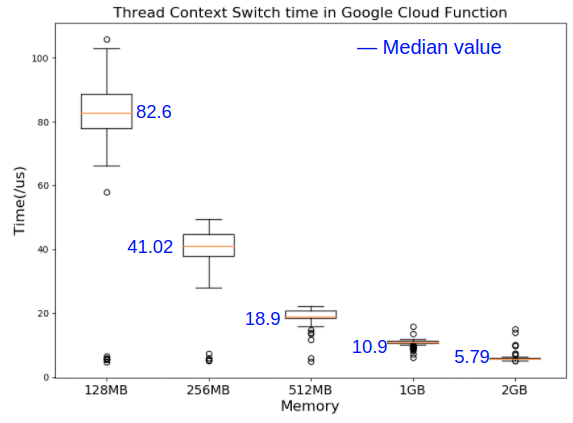
\includegraphics[width=\linewidth]{figure/thread_cloud.png}
	\caption{Thread context switches time in Google Cloud Function}
	\label{fig:thread_cloud}
\end{figure}

\begin{figure}
	\centering
	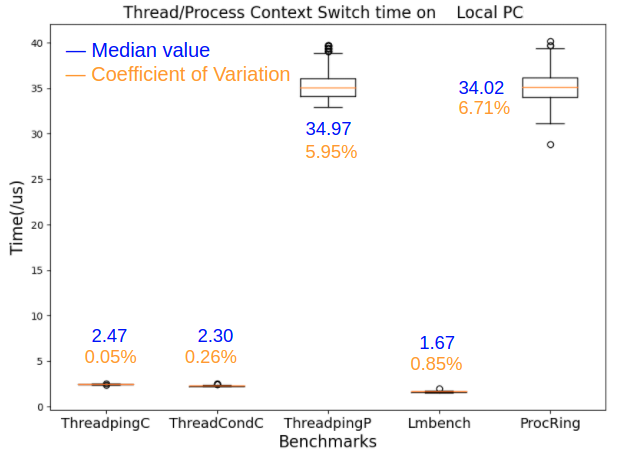
\includegraphics[width=\linewidth]{figure/thread_local.png}
	\caption{Thread/Process context switches time in local PCs}
	\label{fig:thread_local}
\end{figure}

\begin{figure}
	\centering
	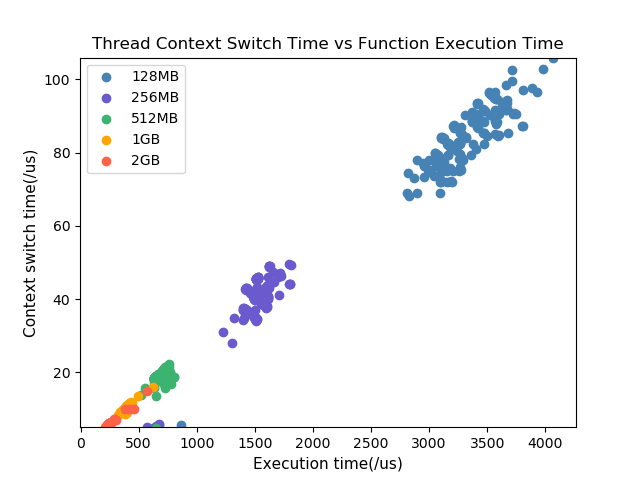
\includegraphics[width=\linewidth]{figure/cxt_vs_exe.png}
	\caption{Thread context switch time vs Function execution time}
	\label{fig:cxt_exe}
\end{figure}
